\section{Company, Sector, and Year-wise Results}
\label{sec:results}

The application results present four reporting levels: one company, selected companies within a sector, the complete financial-sector group, and all recorded sectors. A separate paired-year analysis examines change over time. The database contains 1,164 companies and 1,172 reports, including eight companies with two reports. Company and sector summaries use one score per CIN from the latest available report selected by the export procedure. The following examples connect these summaries with the component counts and source records.

\subsection{One company: evidence and score calculation}
\label{sec:case}

Triveni Turbine Limited provides a worked example with complete score components and a sector comparison. The report ends on 31 March 2026 and contains 1,862 raw facts. Table~\ref{tab:case_facts} presents previous- and current-year values for matched concepts and units. Scope 1 emissions increase, whereas Scope 2 emissions and water withdrawal decrease. The unit tCO2e means tonnes of carbon dioxide equivalent. These different directions illustrate why a broad claim about environmental improvement needs a measure-specific check, including the reporting period and business boundary.

\begin{table}[tbp]
\centering\small
\caption{Previous- and current-year values from Triveni Turbine report record 197. The original concept, unit, and period fields remain linked to each value.}
\label{tab:case_facts}
\begin{tabularx}{\linewidth}{@{}Yrrl@{}}
\toprule\textbf{Filed measure} & \textbf{FY2024--25} & \textbf{FY2025--26} & \textbf{Filed unit}\\\midrule
Scope 1 emissions & 4,142.84 & 5,177.03 & tCO2e\\
Scope 2 emissions & 3,353.61 & 3,169.15 & tCO2e\\
Total water withdrawal & 88,662.28 & 85,611.54 & Kilolitres\\\bottomrule
\end{tabularx}
\end{table}

The score can be reconstructed from the retained records. Completeness is $100(613/1057)=57.99\%$, based on 613 accepted concepts. Among 52 retained concept--text pairs, 33 contain an evidence marker, giving Specificity of 63.46\%. One text segment is flagged as vague, giving Clarity of 98.08\%. Twelve mapped goals produce SDG breadth of 70.59\%. Table~\ref{tab:case_score} applies the fixed weights, yielding $23.196+19.038+19.616+7.059=68.909$, rounded to 68.91. Figure~\ref{fig:company_contributions} shows the weighted component contributions. Within Machinery and Equipment, the company has a sector percentile of 94.4, compared with a mean score of 49.46 across 36 companies.

\begin{table}[tbp]
\centering\small
\caption{Weighted components of the Triveni Turbine score. Each contribution equals the component percentage multiplied by the fixed weight.}
\label{tab:case_score}
\begin{tabularx}{\linewidth}{@{}Yrrr@{}}
\toprule\textbf{Component} & \textbf{Percentage} & \textbf{Weight} & \textbf{Contribution}\\\midrule
Completeness & 57.99 & 0.40 & 23.196\\
Specificity & 63.46 & 0.30 & 19.038\\
Clarity & 98.08 & 0.20 & 19.616\\
SDG breadth & 70.59 & 0.10 & 7.059\\\midrule
\textbf{Transparency Score} & & & \textbf{68.91}\\\bottomrule
\end{tabularx}
\end{table}

\begin{figure}[tbp]
\centering
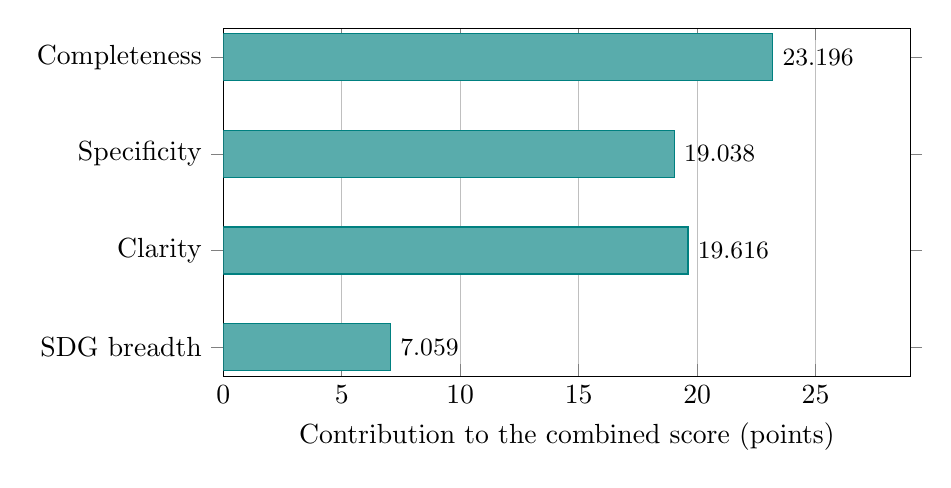
\begin{tikzpicture}
\begin{axis}[width=0.85\linewidth,height=6cm,xbar,bar width=17pt,
  xlabel={Contribution to the combined score (points)},xmin=0,xmax=29,
  symbolic y coords={SDG breadth,Clarity,Specificity,Completeness},ytick=data,xmajorgrids=true,
  nodes near coords,nodes near coords style={font=\small,/pgf/number format/fixed,/pgf/number format/precision=3}]
\addplot[fill=teal!65,draw=teal] coordinates {(7.059,SDG breadth)(19.616,Clarity)(19.038,Specificity)(23.196,Completeness)};
\end{axis}
\end{tikzpicture}
\caption{Weighted contributions to the Triveni Turbine Transparency Score. Each bar equals the component percentage multiplied by the fixed weight; the contributions total 68.91 after rounding.}
\label{fig:company_contributions}
\end{figure}

\FloatBarrier

\subsection{Selected financial companies: component differences}
\label{sec:selected_finance}

The saved Financial Services (excl. Insurance) group contains 94 companies. Table~\ref{tab:financial_selected} presents the four highest and three lowest scores, showing component differences across the score range rather than a random company group. REC Limited scores 67.56, compared with 29.83 for Vardhman Holdings. Specificity is 57.69\% and 2.78\%, respectively, while Completeness is 56.01\% and 35.00\%. The shared formula makes the source of the score difference visible. Business activity, applicable reporting items, and report year remain relevant when interpreting the comparison; Supplementary Table~\ref{tab:supp_financial} retains the complete company records.

\begin{table}[tbp]
\centering\small
\caption{Selected high- and low-scoring financial companies. FY end denotes 31 March of the stated year, reconstructed from the latest report per CIN. Components are percentages; TS is the combined score.}
\label{tab:financial_selected}
\begin{tabularx}{\linewidth}{@{}Yrrrrrr@{}}
\toprule\textbf{Company} & \textbf{FY end} & \textbf{$C$} & \textbf{$Sp$} & \textbf{$Cl$} & \textbf{$G$} & \textbf{TS}\\\midrule
REC & 2026 & 56.01 & 57.69 & 98.08 & 82.35 & 67.56 \\
Mahindra \& Mahindra Financial Services & 2026 & 67.83 & 49.15 & 98.31 & 29.41 & 64.48 \\
YES BANK & 2026 & 60.45 & 46.67 & 92.00 & 70.59 & 63.64 \\
KOTAK MAHINDRA BANK & 2026 & 61.21 & 59.42 & 95.65 & 17.65 & 63.21 \\
Fedbank Financial Services & 2025 & 31.98 & 12.12 & 75.76 & 0.00 & 31.58 \\
Nalwa Sons Investments & 2025 & 31.13 & 10.26 & 74.36 & 0.00 & 30.40 \\
Vardhman Holdings & 2025 & 35.00 & 2.78 & 75.00 & 0.00 & 29.83 \\
\bottomrule
\end{tabularx}
\end{table}

\FloatBarrier
\subsection{The complete financial-sector group}
\label{sec:all_finance}

Across all 94 financial companies, the mean score is 48.17, the median is 49.79, and the standard deviation is 9.88. The median identifies the middle score, while standard deviation describes the spread around the mean. Scores range from 29.83 to 67.56, a difference of 37.73 points. Mean component values are 49.77\% for Completeness, 28.35\% for Specificity, 90.67\% for Clarity, and 16.27\% for SDG breadth. The separation between Clarity and Specificity shows that avoiding vague wording does not necessarily provide concrete evidence.

Table~\ref{tab:all_financial} groups companies into four score bands. Eleven companies score at least 60, while 22 score below 40. Mean Specificity rises from 14.30\% in the lowest band to 47.24\% in the highest. The sector mean is 0.56 points below the overall company mean of 48.73, although the company range shows substantial variation within the sector. The latest report ends in March 2026 for 77 companies and March 2025 for 17 companies. These dates were reconstructed by CIN because the original score export omitted report identifiers, so this comparison uses the latest available reports rather than one common reporting year.

\begin{table}[tbp]
\begin{singlepagetable}
\centering\small
\caption{Financial-sector score distribution across all 94 companies. Component columns report band means. Complete company values and reconstructed dates appear in Supplementary Table~\ref{tab:supp_financial}.}
\label{tab:all_financial}
\begin{tabularx}{\linewidth}{@{}Yrrrrrrr@{}}
\toprule\textbf{Score band} & \textbf{N} & \textbf{Mean TS} & \textbf{Range} & \textbf{$C$} & \textbf{$Sp$} & \textbf{$Cl$} & \textbf{$G$}\\\midrule
60.00--69.99 & 11 & 62.39 & 60.01--67.56 & 61.17 & 47.24 & 95.25 & 47.06 \\
50.00--59.99 & 35 & 54.77 & 50.23--59.84 & 60.69 & 32.94 & 94.07 & 17.98 \\
40.00--49.99 & 26 & 45.22 & 40.57--49.96 & 45.85 & 26.05 & 89.79 & 11.08 \\
Below 40.00 & 22 & 34.05 & 29.83--39.80 & 31.33 & 14.30 & 84.02 & 4.28 \\
\midrule
All financial companies & 94 & 48.17 & 29.83--67.56 & 49.77 & 28.35 & 90.67 & 16.27\\\bottomrule
\end{tabularx}
\end{singlepagetable}
\end{table}

\FloatBarrier
\subsection{All sectors: coverage and score distribution}
\label{sec:all_sectors}

The complete collection contains 1,164 company scores across 72 recorded sectors. The mean is 48.73, the median is 47.25, and scores range from 26.88 to 75.58. Forty-seven sectors contain at least five companies and account for 1,109 scores; the remaining 25 sectors contain 55 companies. Table~\ref{tab:all_sectors} lists the 47 eligible sectors and pools the smaller groups. Supplementary Table~\ref{tab:supp_sectors} provides all 72 sector rows, including medians and group sizes.

Among eligible groups, Warehousing and Transport Support has the highest mean, 54.55 across six companies. Wearing Apparel has the lowest mean, 42.33 across six companies, followed by Education at 42.43 across six companies. The highest and lowest means differ by 12.22 points. Larger groups provide additional context: Chemicals Manufacturing contains 101 companies with a mean of 49.56, Financial Services contains 94 with a mean of 48.17, and Pharmaceuticals contains 65 with a mean of 51.18. Pharmaceuticals scores range from 32.38 to 73.72, compared with 32.18 to 75.34 in Chemicals Manufacturing. These figures describe the saved scores and show variation both within and between recorded sectors.

\begin{table}[p]
\begin{singlepagetable}
\centering
\begingroup
\footnotesize
\setlength{\tabcolsep}{5pt}
\renewcommand{\arraystretch}{1.00}
\caption{Transparency Scores across all 1,164 companies. The 47 sectors with at least five companies are listed separately, and 25 smaller sectors are pooled. SD is the standard deviation. Full sector records appear in Supplementary Table~\ref{tab:supp_sectors}.}
\label{tab:all_sectors}
\begin{tabularx}{\linewidth}{@{}Yrrrr@{}}
\toprule\textbf{Sector or reporting group} & \textbf{N} & \textbf{Mean TS} & \textbf{Range} & \textbf{SD}\\\midrule
Chemicals Manufacturing & 101 & 49.56 & 32.18--75.34 & 9.32 \\
Financial Services (excl. Insurance) & 94 & 48.17 & 29.83--67.56 & 9.88 \\
Pharmaceuticals & 65 & 51.18 & 32.38--73.72 & 10.06 \\
Basic Metals & 60 & 50.80 & 34.61--75.58 & 10.87 \\
Electrical Equipment & 51 & 48.80 & 26.88--67.03 & 9.56 \\
Computer Programming and Information Technology Services & 49 & 50.24 & 32.89--73.98 & 12.25 \\
Non-Metallic Mineral Products & 40 & 50.36 & 35.66--69.20 & 8.69 \\
Food Products Manufacturing & 38 & 47.57 & 30.04--69.86 & 9.60 \\
Motor Vehicles & 37 & 51.76 & 33.29--70.12 & 9.98 \\
Machinery and Equipment & 36 & 49.46 & 35.61--69.67 & 10.06 \\
Rubber and Plastics & 36 & 49.22 & 35.44--73.87 & 9.90 \\
Auxiliary Financial Services & 31 & 47.26 & 27.67--61.39 & 9.08 \\
Electricity, Gas, Steam and AC Supply & 31 & 53.67 & 31.95--74.23 & 11.49 \\
Fabricated Metal Products & 27 & 50.29 & 35.03--65.72 & 8.66 \\
Textiles & 26 & 47.44 & 31.77--67.65 & 10.16 \\
Wholesale Trade & 24 & 45.46 & 28.05--64.86 & 12.39 \\
Civil Engineering & 23 & 48.31 & 31.99--66.15 & 10.84 \\
Retail Trade & 21 & 43.06 & 34.22--56.45 & 6.12 \\
Construction & 20 & 48.73 & 36.58--63.25 & 8.32 \\
Insurance and Pension Funding & 20 & 51.52 & 29.92--64.17 & 10.12 \\
Real Estate Activities & 19 & 47.90 & 35.17--63.42 & 8.78 \\
Human Health Activities & 18 & 46.37 & 33.92--62.86 & 8.12 \\
Information Service Activities & 18 & 47.39 & 33.97--64.19 & 9.71 \\
Computer, Electronic and Optical Products & 17 & 47.46 & 32.93--65.45 & 7.59 \\
Other Transport Equipment & 17 & 50.83 & 37.67--66.89 & 9.39 \\
Other Manufacturing & 16 & 46.11 & 30.59--63.81 & 10.19 \\
Telecommunications & 15 & 50.63 & 36.57--69.19 & 11.43 \\
Accommodation & 14 & 48.67 & 31.28--67.57 & 10.06 \\
Mining and Quarrying & 13 & 47.40 & 29.01--73.16 & 13.27 \\
Beverages Manufacturing & 10 & 47.30 & 34.70--67.71 & 13.18 \\
Other (Division 99) & 10 & 48.39 & 34.80--73.44 & 12.12 \\
Wholesale/Retail Trade - Motor Vehicles & 10 & 49.25 & 37.40--67.92 & 11.47 \\
Architecture and Engineering & 9 & 48.50 & 37.49--64.86 & 10.06 \\
Coke and Refined Petroleum & 9 & 52.32 & 38.20--69.63 & 11.13 \\
Paper Products & 9 & 43.27 & 33.42--48.93 & 4.88 \\
Broadcasting & 8 & 43.65 & 31.66--52.74 & 7.64 \\
Land Transport & 7 & 47.42 & 34.72--63.63 & 10.11 \\
Water Supply and Waste Management & 7 & 43.33 & 36.73--56.76 & 8.29 \\
Wood Products & 7 & 46.18 & 36.16--64.51 & 9.72 \\
Education & 6 & 42.43 & 33.28--55.70 & 7.74 \\
Furniture & 6 & 51.28 & 36.17--65.29 & 9.25 \\
Other Professional/Technical Activities & 6 & 48.43 & 38.73--57.90 & 8.70 \\
Scientific R\&D & 6 & 44.90 & 38.95--52.11 & 5.71 \\
Warehousing and Transport Support & 6 & 54.55 & 37.82--67.03 & 10.34 \\
Wearing Apparel & 6 & 42.33 & 37.17--48.78 & 4.50 \\
Leather Products & 5 & 50.00 & 42.14--58.86 & 7.80 \\
Water Transport & 5 & 48.37 & 38.70--61.22 & 9.75 \\
\midrule
Other 25 small sectors (combined) & 55 & 44.08 & 27.56--70.97 & 8.95\\
\textbf{All 72 sectors} & \textbf{1,164} & \textbf{48.73} & \textbf{26.88--75.58} & \textbf{9.98}\\\bottomrule
\end{tabularx}
\endgroup
\end{singlepagetable}
\end{table}
\FloatBarrier

Within the recorded Pharmaceuticals group, Dabur India scores 73.72 and Kopran scores 32.38, a gap of 41.34 points. Completeness is 73.13\% for Dabur India and 32.92\% for Kopran; Specificity is 57.38\% and 23.68\%, respectively. Clarity exceeds 85\% for 58 of the 65 companies, so differences in coverage and evidence markers remain important even when vague wording is uncommon. Supplementary Table~\ref{tab:supp_pharma} preserves the four highest and three lowest examples with every component.

\FloatBarrier
\subsection{Year-wise changes in the available paired reports}
\label{sec:yearwise}

Eight companies across sectors have reports for both FY2024--25 and FY2025--26. Table~\ref{tab:esaf} compares the paired scores and identifies the component with the largest absolute weighted contribution to each change. Six scores rise and two fall. The group mean increases from 45.17 to 50.40, or 5.23 points. This available-case comparison describes the eight recorded pairs rather than a market-wide trend. Supplementary Table~\ref{tab:supp_paired} retains both report identifiers, year labels, and all component values.

\begin{table}[tbp]
\begin{singlepagetable}
\centering\small
\caption{Paired-year scores for eight companies across sectors. The final column identifies the largest absolute weighted contribution to each score change.}
\label{tab:esaf}
\begin{tabularx}{\linewidth}{@{}Yrrrr@{}}
\toprule\textbf{Company} & \textbf{FY2024--25} & \textbf{FY2025--26} & \textbf{Change} & \textbf{Largest contribution}\\\midrule
Praj Industries & 38.55 & 50.30 & +11.75 & $C$: +9.91 \\
ESAF Small Finance Bank & 42.59 & 54.10 & +11.51 & $C$: +8.10 \\
Sudarshan Colorants & 49.74 & 58.78 & +9.04 & $Sp$: +7.00 \\
Gopal Snacks & 41.30 & 47.29 & +5.99 & $Sp$: +8.53 \\
G R Infraprojects & 35.94 & 38.87 & +2.93 & $Sp$: +3.07 \\
Sudarshan Chemical & 62.95 & 65.32 & +2.37 & $G$: +2.35 \\
VIP Industries & 45.91 & 45.56 & -0.35 & $Cl$: -2.36 \\
SML Mahindra & 44.38 & 42.98 & -1.40 & $Cl$: -1.17 \\
\midrule
Group mean & 45.17 & 50.40 & +5.23 & \na\\\bottomrule
\end{tabularx}
\end{singlepagetable}
\end{table}

ESAF Small Finance Bank illustrates the component calculation over time. Completeness rises from 34.34\% to 54.59\%, Specificity from 30.23\% to 41.30\%, and Clarity from 93.02\% to 93.48\%, while SDG breadth remains 11.76\%. The combined score increases from 42.59 to 54.10. Of the 11.51-point gain, Completeness contributes about 8.10 points, Specificity 3.32, and Clarity 0.09. This decomposition explains the recorded score change using the same fixed weights applied in the company and sector comparisons.

\FloatBarrier
